\chapter{Visual Aids and Displays}
\label{cha:displays}


\section{Science Corner}

\begin{center}
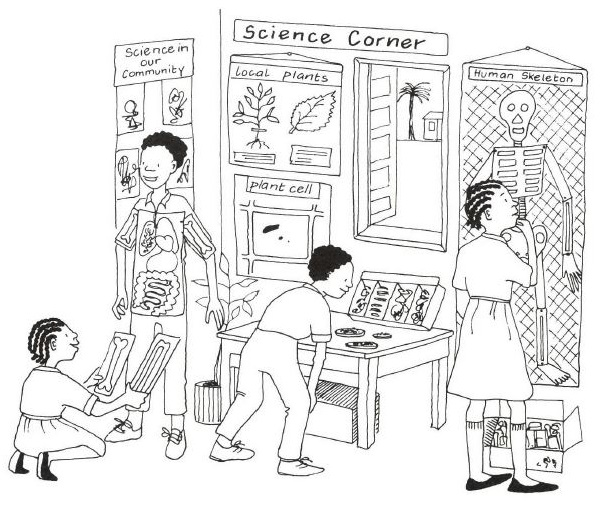
\includegraphics[width=0.99\textwidth]{./img/vso/science-corner.jpg}
\end{center}

\begin{itemize}
\item A table pushed into a corner can be the start of a science corner in
the classroom.
\item A few nails or strips of wood can be added above the table to hang
posters and specimens.
\item The corner could be the focus for science club or science fair activities.
\end{itemize}

\vfill
\pagebreak

%============================================================================================%

\begin{multicols}{2}

\section{Cardboard Box Displays}

\begin{center}
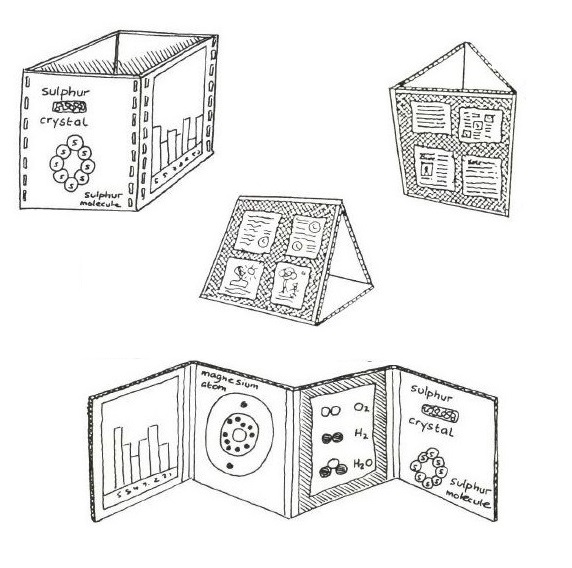
\includegraphics[width=0.49\textwidth]{./img/vso/cardboard-box-2.jpg}
\end{center}

\begin{itemize}
\item Pin display work on the sides of
the box.
\item Sew or tape cardboard sheets
together to make a box.
\item A box can show 8 sides.
\end{itemize}


\subsection{Zigzag Multiboards}

\begin{center}
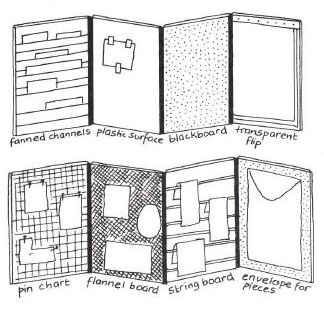
\includegraphics[width=0.49\textwidth]{./img/vso/zigzag.jpg}
\end{center}

\begin{itemize}
\item A portable zigzag board can hold and display many items.
\end{itemize}

\vfill
\columnbreak

\subsection{Portability}

\begin{center}
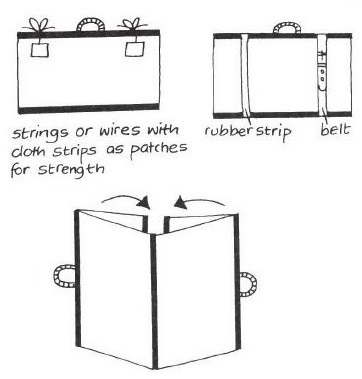
\includegraphics[width=0.4\textwidth]{./img/vso/zigzag-portability.jpg}
\end{center}

\begin{itemize}
\item Fold the outer wings in,
close the board.
\item The boards can be made from
plywood, hardwood or
cardboard.
\item Fastenings can be made from
many materials.
\end{itemize}

%\subsection{Variations}
%
%\begin{center}
%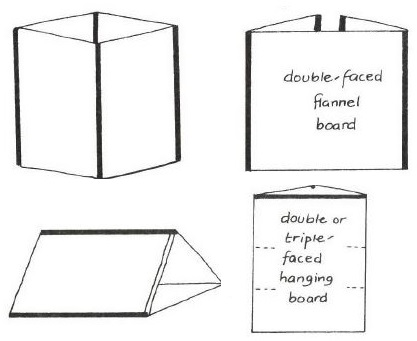
\includegraphics[width=0.45\textwidth]{./img/vso/zigzag-variations.jpg}
%\end{center}
%
%\begin{itemize}
%\item Experiment with different angles and presentation techniques.
%\item Try different combinations in one board.
%\end{itemize}

%============================================================================================%

\section{Hanging Displays}


\subsection{Display Beams and Hooks}

\begin{center}
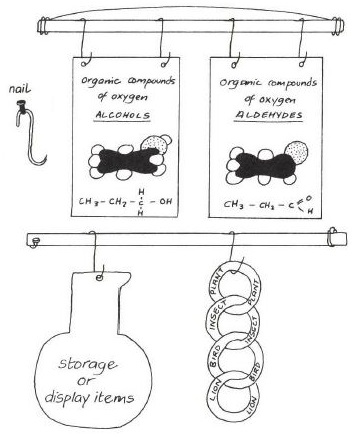
\includegraphics[width=0.49\textwidth]{./img/vso/display-beams-hooks.jpg}
\end{center}

\begin{itemize}
\item Make a beam supported by 2 nails or loops of wire.
It can be hung on the wall, or suspended from a beam.
\item Hooks of wire allow easy and swift display.
\end{itemize}

\subsection{Display Charts}

\begin{center}
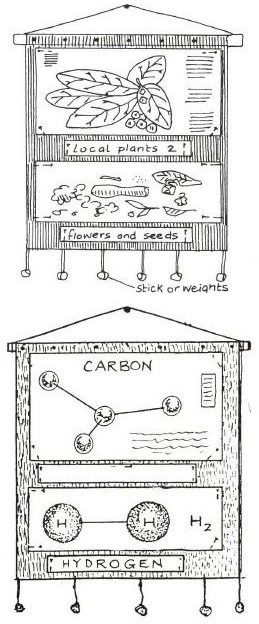
\includegraphics[width=0.4\textwidth]{./img/vso/display-charts-alt.jpg}
\end{center}

\begin{itemize}
\item Display charts can be made
from durable cement bags,
cloth, cardboard boxes, sleeping
mats and blankets.
\item To make the chart hang flat,
attach a strip of wood to the
top and either another strip of
wood or weights to the bottom.
\item Strips at top and bottom will
strengthen the chart and make
it last longer.
\item Attach items to be displayed to
the chart with office pins, cactus
needles or sharpened
matchsticks.
\end{itemize}

%\subsection{Hanging Mats}
%
%\begin{center}
%\includegraphics[width=12cm]{./img/vso/hanging-mats.jpg}
%\end{center}

\columnbreak

\subsection{String Display Lines}

\begin{center}
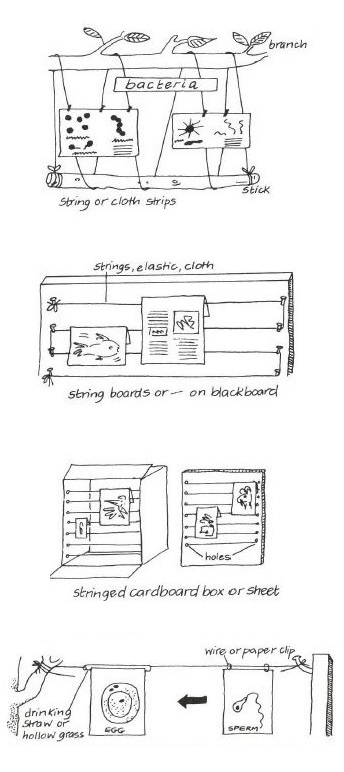
\includegraphics[width=0.49\textwidth]{./img/vso/string-display.jpg}
\end{center}

\begin{itemize}
\item String can be used in many ways to display items. Some ideas are given here.
\item Hollow tubes, e.g. drinking
straws, or paper clips will allow
the display to slide up and
down the string.
\end{itemize}

\vfill
\columnbreak

\subsection{Carrier Bag Display}

\begin{center}
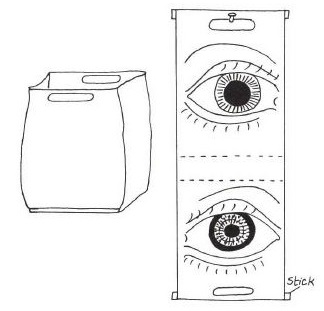
\includegraphics[width=0.4\textwidth]{./img/vso/carrier-bag.jpg}
\end{center}

\begin{itemize}
%\item Open out a plastic carrier bag
%and tidy the edges.
\item Attaching a wooden stick at the
top and bottom of the carrier
bag adds strength and makes it
hang flat.
\item Permanent or temporary marker pens can be
used to draw onto the plastic.
\item Use Sellotape tabs to attach
pieces to the display chart.
These can be movable pieces.
\end{itemize}

%============================================================================================%

%\section{Fold-Away Posters}
%
%\begin{center}
%\includegraphics[width=12cm]{./img/source/fold-away-poster.jpg}
%\end{center}

%============================================================================================%

\section{Transparent Flip-Sheets}

\begin{center}
\includegraphics[width=0.49\textwidth]{./img/vso/transparent-display.jpg}
%\includegraphics[width=0.49\textwidth]{./img/source/transparent-display.jpg}
\end{center}

\begin{itemize}
\item You will need plastic sheets (from a stationery store), a bar of wood and some nails or pins.
%\item You can put together as many sheets as you want.
% ref in Bio circulation overlay chart (VSO 33)
\item Lift up different sheets to show the combinations you want.
\end{itemize}

\vfill
\columnbreak

%============================================================================================%

\section{Clothing Posters}

\begin{center}
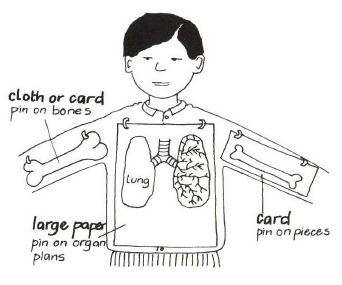
\includegraphics[width=0.45\textwidth]{./img/vso/clothing-poster.jpg}
\end{center}

\begin{itemize}
\item Body organs could be drawn,
painted or pinned onto gloves,
T-shirts or trousers.
\end{itemize}

%\vfill
%\columnbreak

%============================================================================================%

\section{Magnet Boards}

\begin{center}
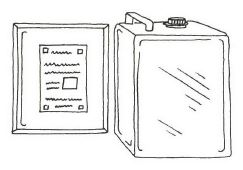
\includegraphics[width=0.4\textwidth]{./img/vso/magnet-board.jpg}
\end{center}

\begin{itemize}
\item Use a thin metal sheet. Paint it black to act as a blackboard too.
\item Metal could come from old cans or car panels, fridge doors, filing
cabinets, steel shelves, flattened corrugated sheet, storage trunks.
\item Tape over the edges of the sheet, or hammer the edges over for
safety.
\item Magnetize small pieces of metal to attach pictures to
the metal sheet.
% ref in Physics to magnetization
\item Painting the metal pieces white makes them less noticeable. Glue the
magnetic pieces to the back of pictures used regularly.
\end{itemize}


\end{multicols}